
\begin{frame}{Transfer Function Review}
        A \textbf{\emph{transfer function}} of a circuit or system describes the \textcolor{red}{output response} to an \textcolor{red}{input excitation} as a function of the angular frequency $\omega$.
        \begin{center}
            $H(\omega) = \frac{V_{out}(\omega)}{V_{in}(\omega)}$
        \end{center}
    \end{frame}

    \begin{frame}{RC Circuits}
        \begin{columns}
            \begin{column}{0.5\textwidth}
            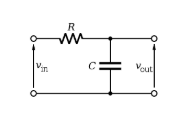
\includegraphics[]{./images/rc-circuits_1.png}
                \vspace{2ex}
                $H(\omega) = \frac{1}{1 + j\omega RC}$
                \vspace{2ex}

                \textbf{Low pass:} $\lim_{\omega\to\infty} H(\omega) = 0, H(0) = 1$
            \end{column}
            \begin{column}{0.5\textwidth}
            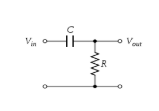
\includegraphics[]{./images/rc-circuits_2.png}
                \vspace{2ex}
                $H(\omega) = \frac{j\omega RC}{1 + j\omega RC}$
                \vspace{2ex}

                \textbf{High pass:} $\lim_{\omega\to\infty} H(\omega) = 1, H(0) = 0$
            \end{column}
        \end{columns}
    \end{frame}
    
    \begin{frame}{Bode Plot Review}
        $V[dB] = 20\log_{10}(\frac{V}{V_0})$
        \begin{itemize}
            \item Bode plots provide a way for us to easily visualize the output response of our system, depending on the input frequency $\omega$. 
            \item Because Bode plots are in log scale for $\omega$, we are able to take advantage of the properties of logs.
            \begin{itemize}
                \item $G = XY \implies G[dB] = X[dB] + Y[dB]$
                \item $G = \frac{X}{Y} \implies G[dB] = X[dB] - Y[dB]$
            \end{itemize}
        \end{itemize}
        Hence, we can break our transfer function H($\omega$) into a product of familiar transfer functions (simple poles, quadratic zeros, etc. - “functional forms”), graph them out individually, and then add them together on the graph.  
    \end{frame}
    \begin{frame}{Bode Plot Review}
        \begin{itemize}
            \item We want to be able to plot the transfer function as a function of the frequency $\omega$. 
            \item However, it’s a complex valued function so it’s easier to have a plot for the magnitude and one for the phase. 
            \item Because the magnitude plot is in log scale, and the phase plot is in semi-log scale we are able to take advantage of the properties of logs. 
            \begin{itemize}
                \item $\log(XY) = \log(X) + \log(Y)$
            \end{itemize}
            \item Hence, we can break our transfer function H($\omega$) into a product of familiar transfer functions (simple poles, quadratic zeros, etc. - “functional forms”), graph them out individually, and then add them together on the graph.
        \end{itemize}
    \end{frame}
    \begin{frame}{Bode Plot Steps}
        \begin{enumerate}
            \item Break transfer function into product of functional forms
            \begin{enumerate}
                \item $H(\omega) = \frac{n(\omega)}{d(\omega)} = \frac{(j\omega)^n\alpha_{n} + (j\omega)^{n-1}\alpha_{n-1} + \ldots  + j \omega \alpha_1 + \alpha_0}{(j\omega)^n\beta_{n} + (j\omega)^{n-1}\beta_{n-1} + \ldots  + j \omega \beta_1 + \beta_0} = \kappa \frac{(j\frac{\omega}{\omega_{z1}} +1)(j\frac{\omega}{\omega_{z2}} +1) \ldots}{(j\frac{\omega}{\omega_{\rho1}} +1)(j\frac{\omega}{\omega_{\rho2}} +1) \ldots}$
            \end{enumerate}
            \item Graph each transfer function individually
            \item Add them up on the graph (thanks to log scale)
            \begin{enumerate}
                \item 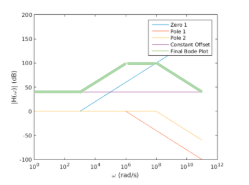
\includegraphics[scale=0.5]{./images/bode-plot-steps-1.png}
            \end{enumerate}
        \end{enumerate}
    \end{frame}
    \begin{frame}{RC Circuits, revisited}
        \begin{columns}
            \begin{column}{0.5\textwidth}
                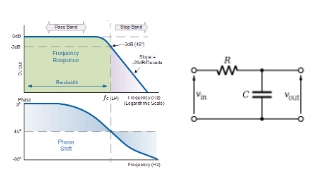
\includegraphics[scale=0.75]{./images/Rc-circuits-revisited-1.png}\\
                $H(\omega) = \frac{1}{1 + j\omega RC}$
            \end{column}
            \begin{column}{0.5\textwidth}
                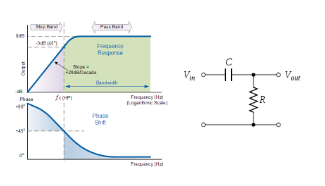
\includegraphics[scale=0.75]{./images/rc-circuits-revisited-2.png}\\
                $H(\omega) = \frac{j\omega RC}{1 + j\omega RC}$
            \end{column}
            
        \end{columns}
    \end{frame}
    \begin{frame}{Important Functional Forms}
        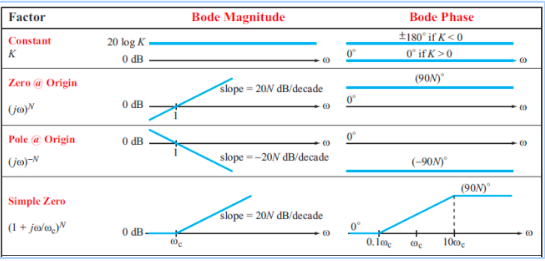
\includegraphics[scale=0.75]{./images/important-functional-forms-1.png}
    \end{frame}
    \begin{frame}{Important Functional Forms}
        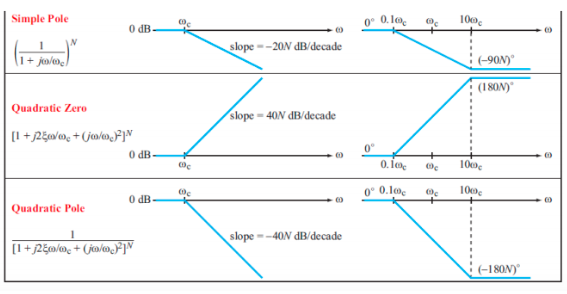
\includegraphics[scale=0.75]{./images/important-functional-forms-2.png}
    \end{frame}
    \begin{frame}{Practice Problem}
        $$H(\omega) = \frac{\frac{j\omega}{10} + 100}{1 + \frac{(j\omega)^2}{10^14} + \frac{j\omega}{10^8} + \frac{j\omega}{10^6}}$$\\
        \begin{center}
            Draw the Bode plot for this transfer function.
        \end{center}
    \end{frame}
    \begin{frame}{}
        \begin{columns}
            \begin{column}{0.5\textwidth}
                $$H(\omega) = \frac{\frac{j\omega}{10} + 100}{1 + \frac{(j\omega)^2}{10^14} + \frac{j\omega}{10^8} + \frac{j\omega}{10^6}}$$\\
                $$=\frac{100(\frac{j\omega}{10^3}+1)}{(\frac{j\omega}{10^6}+1)(\frac{j\omega}{10^8}+1)}
                $$
            \end{column}
            \begin{column}{0.5\textwidth}
                Main idea: break our transfer function into the product of standard forms- a constant, one zero, and two poles
            \end{column}
        \end{columns}
        
    \end{frame}
    \begin{frame}{}
        \begin{columns}
            \begin{column}{0.25\textwidth}
                Final Result
            \end{column}
            \begin{column}{0.75\textwidth}
                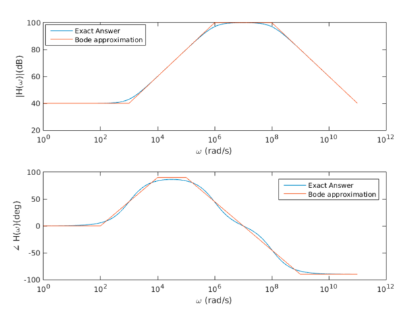
\includegraphics[scale=0.75]{./images/practice-problem.png}\\
            \end{column}
        \end{columns}
    \end{frame}
    \begin{frame}{Common Filters and their Bode Plots}
        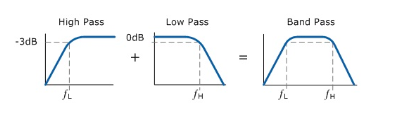
\includegraphics[]{./images/common-filter-bode-plot.png}\\
        In the high pass filter, the frequencies greater than the corner frequency have a gain of 0dB (so they aren’t changed), while frequencies less than the corner frequency have a gain < 0dB (so they are multiplied by something less than 1). \\
        In the lowpass filter, the opposite is true.
    \end{frame}
    \begin{frame}{Design Problem}
        Design an active high pass filter with cutoff frequency of 1KHz and a gain of 1000.\\
        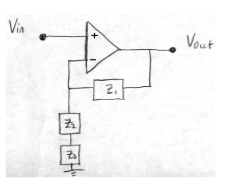
\includegraphics[scale=0.65]{./images/design-problem-summary.png}\\
        \begin{itemize}
            \item Hint 1:  Find the transfer function of the following circuit.
            \item Hint 2: Which transfer function is a high pass filter?
            \begin{itemize}
                \item $H_1(\omega) = 1 + \frac{j\omega R_1C}{1 + j\omega R_2C}$
                \item $H_2(\omega) = 1 + \frac{R_1R_2}{1 + j\omega R_1C}$
            \end{itemize}
            \item Hint 3: What is the impedance of a resistor in series with a capacitor?
            \item Hint 4: Replace the Z’s with resistors/capacitors/wires/open circuits.
        \end{itemize}
    \end{frame}
    \begin{frame}{Design Problem: Hint 1}
        \begin{itemize}
            \item Step 1: Apply the golden rules of Op. Amps. This means that $V^+ = V^-$.
            \item Step 2: By ohm’s law, we can calculate the current from V- to ground.
            \begin{itemize}
                \item $I = \frac{V_{in}}{Z_2 + Z_3}$
            \end{itemize}
            \item Step 3: By Ohm’s law, we can calculate the output voltage.
            \begin{itemize}
                \item $V_{out} = V_{in}(1 + \frac{Z_1}{Z_2 + Z_3})$
            \end{itemize}
        \end{itemize}
    \end{frame}
    \begin{frame}{Design Problem: Hint 2 + Hint 3}
        \begin{itemize}
            \item The high pass filter transfer function is: $H_1(\omega) = 1 + \frac{j\omega R_1C}{1 + j\omega R_2C}$
            \item To more easily separate the gain from the frequency filtering, we can approximate it as (at high frequencies): $H_1(\omega) = \frac{R_1}{R_2}(\frac{j\omega R_2C}{1 + j\omega R_2 C})$
            \item A resistor in series with a capacitor has impedances of: $R + \frac{1}{j\omega C} = \frac{j \omega RC +1}{j\omega C}$
        \end{itemize}
    \end{frame}
    \begin{frame}{Design Problem: Summary of Hints}
    Now, use all of the earlier hints to get a high pass filter!\\
    (Cutoff Frequency is 1KHz, gain of 1000)\\
    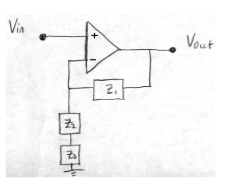
\includegraphics[scale=0.75]{./images/design-problem-summary.png}\\
    $V_{out} = V_{in}(1 + \frac{Z_1}{Z_2+Z_3})$\\
    $H_1(\omega) = 1 + \frac{j\omega R_1 C}{1 + j \omega R_2 C}$ \\
    $R + \frac{1}{j\omega C} = \frac{j \omega RC + 1}{j \omega C}$
    \end{frame}
    \begin{frame}{Design Problem Solution}
        We implement the circuit such that it has the transfer function of :\\
        $$H_1(\omega) = 1 + \frac{j\omega R_1C}{1 + j\omega R_2C}$$\\
        To meet our specifications: \\
        $$\frac{R_1}{R_2} = 1000$$ \\
        $$R_2C = \frac{1}{2\pi(1000)}$$\\
        One Possible Solution: \\
        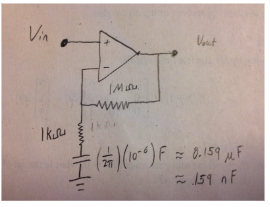
\includegraphics[scale=0.65]{./images/design-problem-solution.png}
    \end{frame}
